% !TEX TS-program = pdflatex
% !TEX encoding = UTF-8 Unicode

%%% DOCUMENT DEFINITIONS
\documentclass[11pt, french]{article} % use larger type; default would be 10pt
\usepackage[utf8]{inputenc} % set input encoding (not needed with XeLaTeX)

%%% PAGE DIMENSIONS
\usepackage{geometry} % to change the page dimensions
\geometry{a4paper} % or letterpaper (US) or a5paper or....
\geometry{margin=2cm} % for example, change the margins to 2 inches all round

%%% PACKAGES
\usepackage{graphicx} % support the \includegraphics command and options
\usepackage{booktabs} % for much better looking tables
\usepackage{array} % for better arrays (eg matrices) in maths
\usepackage{paralist} % very flexible & customisable lists (eg. enumerate/itemize, etc.)
\usepackage{verbatim} % adds environment for commenting out blocks of text & for better verbatim
\usepackage{subfig} % make it possible to include more than one captioned figure/table in a single float
\usepackage{amsmath}
\usepackage[frenchb]{babel}

\usepackage{picins,caption}
\usepackage{wrapfig}
\usepackage{url}

%%% HEADERS & FOOTERS
%\usepackage{fancyhdr} % This should be set AFTER setting up the page geometry
%\pagestyle{fancy} % options: empty , plain , fancy
% Rapport projet pluridisciplinaire : etude thermique du pont en H
% : Xavier Galzin, Stanislas Bertrand, Romain Desille, Frédéric Meslin

\title{\textsc{Projet Pluridisciplinaire} \\ Solution Numérique \\
\begin{minipage}[c][20cm][c]{15cm}
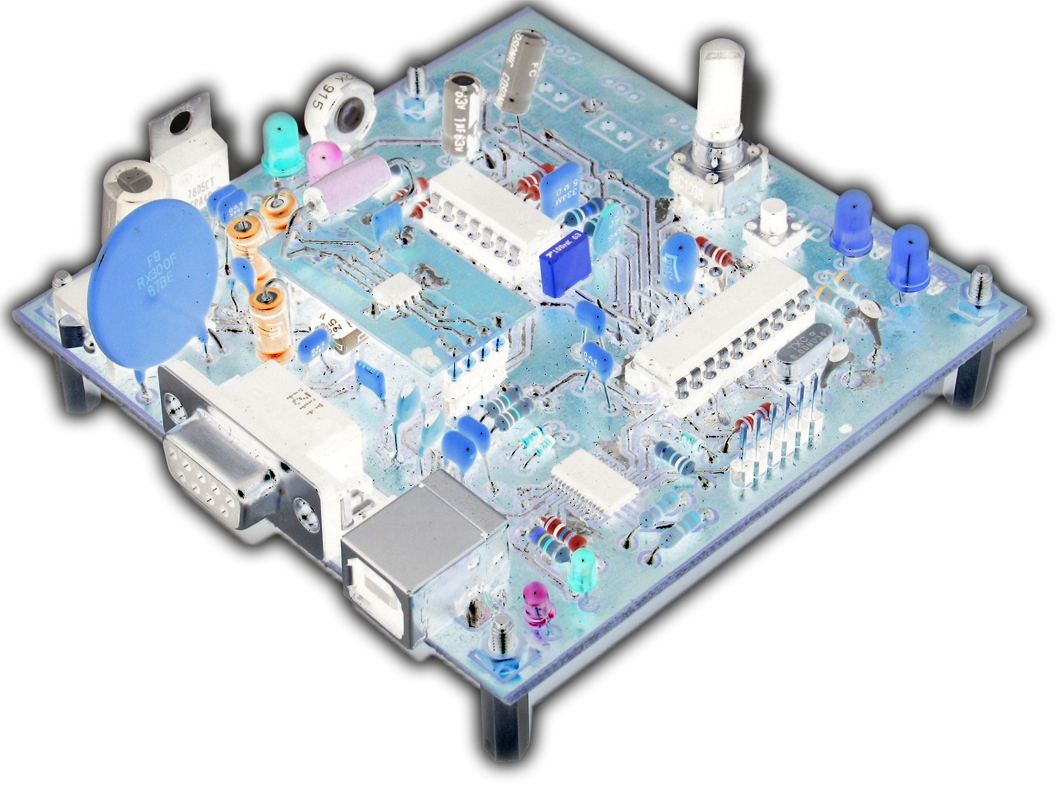
\includegraphics[width=15cm]{../Photos/CarteFrontInv.png}
\end{minipage}}
\author{Xavier GALZIN, Stanislas BERTRAND, Romain DESILLE, Frédéric MESLIN}
\date{\today}

\begin{document}
\maketitle

\pagebreak
\tableofcontents

\pagebreak
\section*{Introduction}
Xavier

\section{Communication}
Fred
\section{Interface}
Romain
\section{Changement de Puissance}
Xavier
\section{Correction Numérique}

Difference avec le rapport d'auto
-> Foh vers Zoh
-> Fréquence de travail

Questions / causes probables :
-> est-ce que le gain de l'avance de phase compte ( analogique ) ?
-> mauvais correcteur
-> mauvais modèle
-> mauvais calcul -> saturation, écretage, arondis

Utilisation d'un outils :
-> suivit des calculs via la série ( diff, avance de phase, sortie )

dernière seance
-> 1 gain du montage différentiel
-> 2 validation avec matlab de la répartition du gain ( av ph, num)
-> 3 validation avec l'asservissement numerique du mercredi du solex
-> 4 essaye d'amélioration de l'asservissement numérique


\section{Répartition des gains}
Xavier - Fred
\subsection{Correcteur Analogique}
\subsection{Correcteur Numérique}
\section*{Conclusion - Evolution}
Xavier

\end{document}

